\documentclass[tikz,border=5pt]{standalone}
\usepackage{amsmath,amssymb}
\usepackage{tikz}
\begin{document}
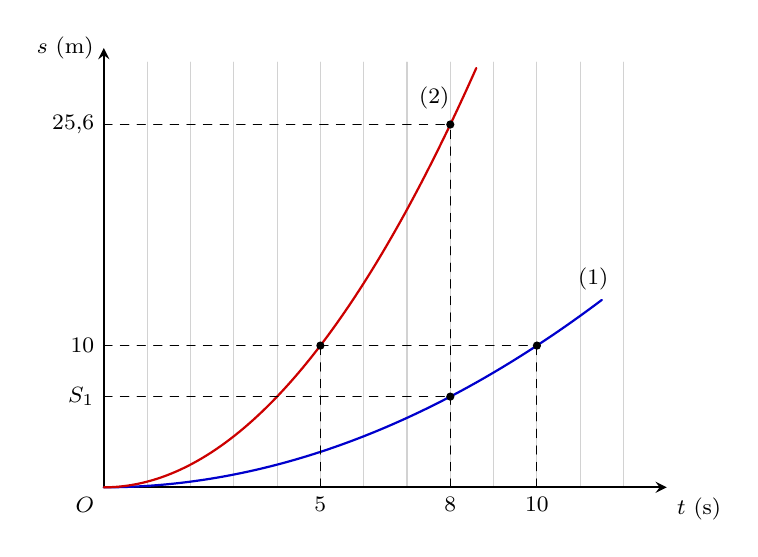
\begin{tikzpicture}[>=stealth, line join=round, line cap=round, font=\footnotesize, xscale=0.55, yscale=0.18]
	% Đường lưới dọc
	\foreach \x in {1,2,...,12} {
		\draw[gray!35, thin] (\x, 0) -- (\x, 30);
	}
	% Hệ trục tọa độ
	\draw[->, thick] (0, 0) -- (13, 0) node[below right] {$t\text{ (s)}$};
	\draw[->, thick] (0, 0) -- (0, 31) node[left] {$s\text{ (m)}$};
	\node[below left] at (0, 0) {$O$};
	% Đồ thị (1) và (2)
	\draw[thick, blue!80!black, samples=100, domain=0:11.5] plot (\x, {0.1*\x*\x});
	\draw[thick, red!80!black, samples=100, domain=0:8.6] plot (\x, {0.4*\x*\x});
	\node[above] at (11.3, 13.2) {$(1)$};
	\node[left] at (8.2, 27.5) {$(2)$};
	% Đường gióng
	\draw[dashed, thin] (0, 6.4) -- (8, 6.4);
	\draw[dashed, thin] (0, 10) -- (10, 10);
	\draw[dashed, thin] (0, 25.6) -- (8, 25.6);
	\draw[dashed, thin] (5, 0) -- (5, 10);
	\draw[dashed, thin] (8, 0) -- (8, 25.6);
	\draw[dashed, thin] (10, 0) -- (10, 10);
	% Nhãn trục
	\node[left] at (0, 6.4) {$S_1$};
	\node[left] at (0, 10) {$10$};
	\node[left] at (0, 25.6) {$25{,}6$};
	\node[below] at (5, 0) {$5$};
	\node[below] at (8, 0) {$8$};
	\node[below] at (10, 0) {$10$};
	% Điểm
	\foreach \p in {(8,25.6), (5,10), (10,10), (8,6.4)}
		\fill[black] \p circle (2.7pt and 8.3pt);
\end{tikzpicture}
\end{document}
